\clearpage
\begin{center}{\large\bfseries The shell theorem, the cored alternative and your thin shell}\end{center}
\vspace{-4pt}
By Newton's shell theorem, matter arranged symmetrically about the CoE pulls a source at radius $r$ as if everything inside $r$ sat at the centre, and matter outside $r$ exerts no net pull. Three rules follow for your picture. First, any symmetric distribution inside $D-R$ acts on every source we see as a single point mass at the CoE, so its profile cannot be measured, only its total mass (and, in the integrated model, the depth of the potential the sources climbed out of). Second, symmetric matter beyond $D+R$ pulls on nothing we see, so its density is free. Third, only matter between $D-R$ and $D+R$ changes across the visible sphere, so for the density there to be uniform, a constant-density shell must be at least $2R$ thick, from $D-R$ to $D+R$. Inside such a shell $g=\tfrac{4\pi}{3}G\rho_s r+G(M_c-M_{\rm hole})/r^2$ with $M_{\rm hole}=\tfrac{4\pi}{3}\rho_sR_{\rm in}^3$. The linear term is isotropic, so in the field today the net central mass $M_c-M_{\rm hole}$ must be positive, or the tidal pattern reverses.

The time-integrated model softens that last rule. The sources start at 1\% of their present scale and move out through the shell, which is fixed in space. The force always uses the mass inside each particle's radius at that moment, so a source spends most of the age inside the empty hole, where only $M_c$ pulls, and enters the shell only in roughly the last $R/D$ of the age (15--30\%). Because the core acted alone for most of that history, your thin shell with a core fits with the usual $\ell_0\approx13^\circ$ even though its net central mass is negative (Table~\ref{tab:alt}). With no core the pattern turns by about $90^\circ$ ($\ell_0=105$--$108^\circ$), as the negative-mass argument predicts, and the fit weakens.

The cored profile $\rho\propto1/(1+(r/L)^2)$, the equal-mass-shell picture with $\rho\propto1/r^2$ far out, is a live alternative. On its own its contrast is about $4R/D$, so it meets $\delta\le2\%$ only at $D=200R$, where $R^2=0.809$. With the LCDM-equivalent background the limit is met at $D=10.8R$ ($D=155$~Gpc, $L=1.6$~Gpc), with $R^2=0.843$. Allowing $D/R$ above the earlier cap of 10 raised this from 0.830. The cored fits are 13.0--13.6 Gyr old, and bound only with the $\Omega=0.3$ background. Your thin shell hugging the visible sphere gives the best $R^2$ of any model so far, 0.909 (0.987 against $A_F$), at $D=94$~Gpc. It is bound and 13.8 Gyr old, but it needs $\Omega_s=1.01$, about 20 times the baryon density. At baryon density it fits as well as the best real-matter model ($R^2=0.893$) but leaves Earth unbound. Moving the shell edges out by $0.1R$ changes $R^2$ by less than 0.001.

\begin{table}[h]\centering\scriptsize\setlength{\tabcolsep}{2.2pt}
\caption{Alternatives to the best real-matter fit, all with $\ell_0$ free, sky-normalised and your $p=1$ convention. Lengths in Gpc. $M$ is all gravitating mass inside $D$. $\Omega$ is the shell or background density; ``LCDM'' is the LCDM-equivalent 0.3 and ``baryons'' is 0.05. Thin shells run from $D-R$ to $D+R$, so their contrast across the sphere is zero. $r_s/D$ uses $r_s=2GM(<D)/c^2$.}\label{tab:alt}
\begin{tabular}{llccllcccccccc}\toprule
Model & Matter & $D/R$ & $D$ & Shape [Gpc] & $M$ [$M_\odot$] & $\Omega$ & $\ell_0$ & $R^2_{\rm Migkas}$ & $R^2_{A_F}$ & $\delta$ [\%] & $(v/v_{\rm esc})^2$ & Age & $r_s/D$\\\midrule
ALTROWS
\bottomrule\end{tabular}\end{table}
\vspace{-6pt}
\begin{figure}[h]\centering
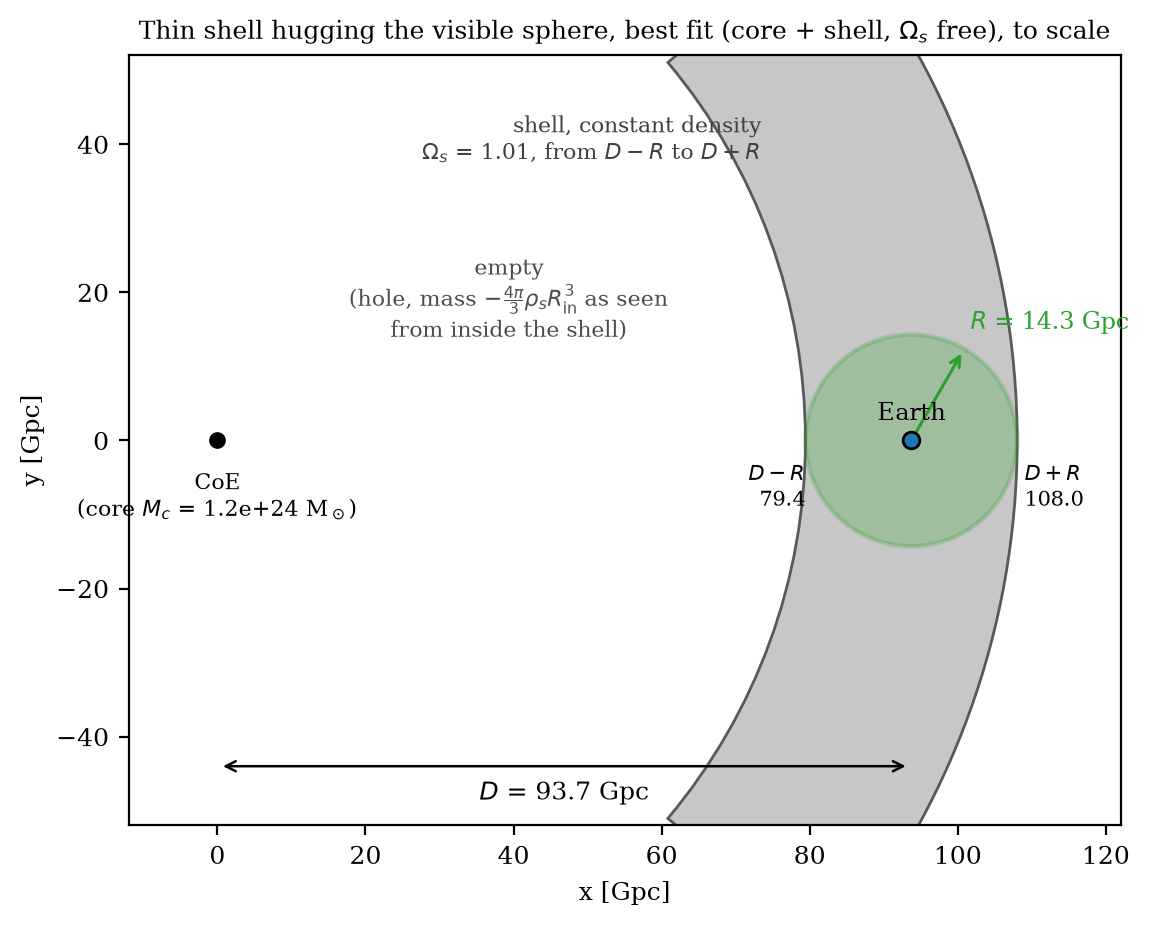
\includegraphics[width=0.49\textwidth]{thin_shell_drawing.png}\hfill
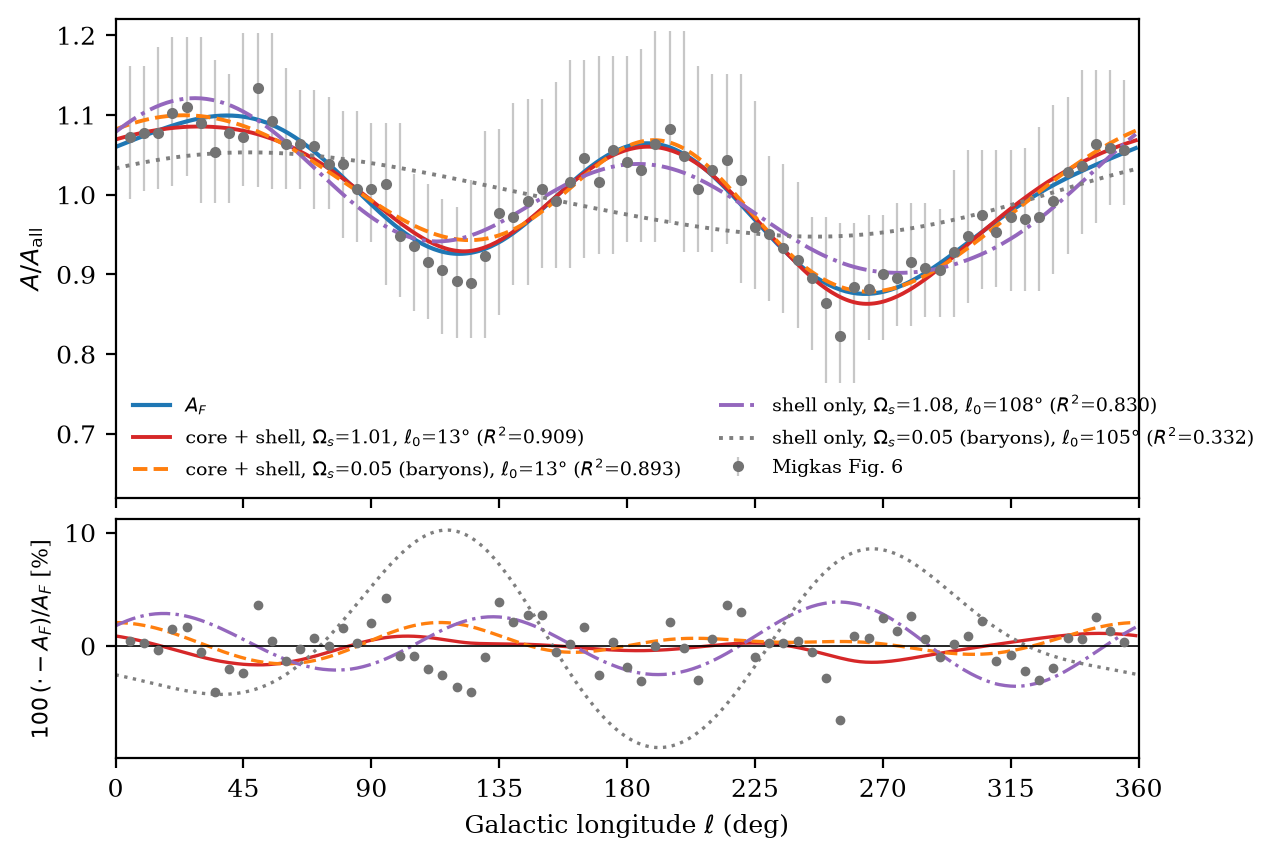
\includegraphics[width=0.49\textwidth]{thin_shell_Achart.png}
\caption{Left: your thin shell, to scale, at its best fit (core plus shell with $\Omega_s$ free). The shell of constant density runs from $D-R$ to $D+R$, and the interior is empty apart from the core. Right: thin-shell fits against the Migkas points and $A_F$. With no core, the pattern turns by about $90^\circ$.}\label{fig:thin}
\end{figure}
